% !TEX root= ../main.tex
\externaldocument{general_trimming}
\externaldocument{odd_paths}
\externaldocument{odd_vels}
\section{Inductive definitions}
\label{sec:Inductive definitions}
All the graph structures presented in this chapter so far can easily be defined inductively.
For instance, given some graph $\mathbf{G}=(G,N)$, let $V_1 \subseteq G \times G$ denote the set of all pairs of vertices related by our original vel-definition (Definition~\ref{def:vel}) where `trimmed' meant strictly non-branching.

We can define $V_1$ inductively in the following way, with $a$ and $b$ being arbitrary vertices from $G$.
\begin{align}
  \textbf{(BC):}&\quad N(a,b) \vee N(b,a) &\Rightarrow  V_1(a,b)\\
  \textbf{(IS):}&\quad \exists c \in N(a): (N(c) =\{d\} \wedge V_1(d,b)) &\Rightarrow V_1(a,b)
\end{align}
The symmetry in the base case is what makes this a definition of a vel and not a path, while the trimmed-ness gets expressed by the restrictions we set on vertex $c$.

Adding the new weaker trimming-restriction is now easy.
Let $V_2 \subseteq G \times G$ be the set of all pairs of vertices related by our new vel-definition.
$V_2$ can be defined inductively in the following way, again with $a$ and $b$ as arbitrary vertices from $G$.
\begin{align}
  \textbf{(BC):}&\quad N(a,b) \vee N(b,a) &\Rightarrow V_2(a,b)\label{eq:V2_BC}\\
  \textbf{(IS):}&\quad \exists c \in N(a):
  \left ( \begin{tabular}{l}
  $\exists d \in N(c): V_2(d,b) \quad \wedge$\\
  $\forall d \in N(c): V_2(d,b) \vee V_2(d,a) \vee V_2(d,d)$
  \end{tabular} \right )
  &\Rightarrow V_2(a,b)\label{eq:V2_IS}
\end{align}
Using the definition above, the fact that $V_2(a,b) \;\Rightarrow\; \vdash \ol{ab}$ can be proven inductively, showing that $V_2$ satisfies implication (1):
\begin{proof}
  Given a graph $G$ with two vertices $a$ and $b$ such that $V_2(a,b)$:

  Base case:
  If $N(a,b)$ or $N(b,a)$, then the NAND-clause $\ol{ab}$ will be an axiom and thus trivially provable.

  Inductive step:
  The existence of a vertex $c \in N(a)$ gives us that the NAND-clause $\ol{ac}$ is an axiom.
  Letting $D$ denoting the set $N(c)$ we also have that the OR-clause $cD$ is an axiom.
  This gives us the following incomplete proof:\par
  \begin{figure}[!h]
    \centering
    \begin{prooftree*}
      \Hypo{\ol{ac}}
      \Hypo{\dots}
      \Infer[right label=$cD$]2{\ol{ab}}
    \end{prooftree*}
    \caption{}
    \label{fig:proof_v2_partial}
  \end{figure}
  Let $D_b$, $D_a$ and $D_d$ be subsets of $D$ such that for any $d \in D$:
  \begin{align}
    d \in D_b \Leftrightarrow V_2(d,b),\quad d \in D_a \Leftrightarrow V_2(d,a),\quad d \in D_d \Leftrightarrow V_2(d,d)
  \end{align}
  The current situation is illustrated in Figure~\ref{fig:v2_situation}\par
  \begin{figure}[!h]
    \centering
    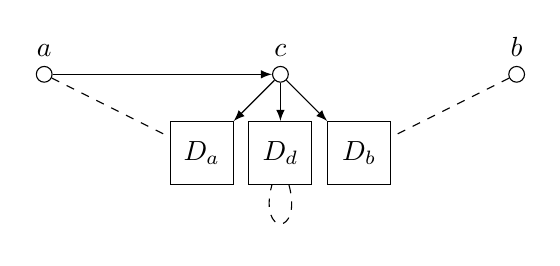
\begin{tikzpicture}
      [
      point/.style={circle,draw,inner sep=0pt,minimum size=2mm},
      collection/.style={rectangle,draw,inner sep=0pt,minimum height=8mm, minimum width= 8mm}
      ]
      \node (a) at (0,1) [point, label=above:$a$] {};
      \node (b) at (6,1) [point, label=above:$b$] {};
      \node (c) at (3,1) [point, label=above:$c$] {};
      \node (Da) at (2,0) [collection] {$D_a$};
      \node (Db) at (4,0) [collection] {$D_b$};
      \node (Dd) at (3,0) [collection] {$D_d$};
      \draw [-latex] (c) to (Da);
      \draw [-latex] (a) to (c);
      \draw [-latex] (c) to (Db);
      \draw [-latex] (c) to (Dd);
      \draw [dashed] (a) to (Da);
      \draw [dashed] (b) to (Db);
      \draw [dashed, loop below] (Dd) to (Dd);
    \end{tikzpicture}
    \caption{The inductive case of a $V_2$ construction.
    Boxes represents sets of vertices.
    An edge between a vertex and a box represents a set of edges from the vertex to each of the vertices in the set.}
    \label{fig:v2_situation}
  \end{figure}
  The inductive part of the $V_2$ definition (\ref{eq:V2_IS}) reveals two properties of the sets $D_b$, $D_a$ and $D_d$:
  \begin{itemize}
    \item The set $D_b$ is nonempty, since $\exists d \in N(c): V_2(d,b)$.
    \item $D_b \cup D_a \cup D_d = D$, since $\forall d \in N(c): V_2(d,b) \vee V_2(d,a) \vee V_2(d,d)$.
  \end{itemize}
  The induction hypothesis lets us assume the provability of the following sets of NAND-clauses:
  $\{ \ol{db} \;|\; d \in D_b \},\{ \ol{da} \;|\; d \in D_a \},\{ \ol{d} \;|\; d \in D_d \}$.
  Inserting these clauses into the incomplete proof from Figure~\ref{fig:proof_v2_partial} results the following proof:\par
  \begin{figure}[!h]
    \centering
    \begin{prooftree*}
      \Hypo{\ol{ac}}
      \Hypo{ \{ \ol{db} \;|\; d \in D_b \} }
      \Hypo{ \{ \ol{da} \;|\; d \in D_a \} }
      \Hypo{ \{ \ol{d} \;|\; d \in D_d \} }
      \Infer[right label=$cD$]4{\ol{ab}}
    \end{prooftree*}
    \caption{}
    \label{fig:proof_v2}
  \end{figure}
The nonemptiness of $D_b$ gives us the existence of a $b$ in the premise, while he fact that $D_b \cup D_a \cup D_d = D$ guarantees that each atom in the OR-clause $D$ has a match in a NAND-clause.

The proof is thus valid, finishing the inductive step and ultimately proving the fact that $V_2(a,b) \Rightarrow \vdash \ol{ab}$.
\end{proof}
Having that $V_2$ satisfies implication (1), if one could show that it also satisfies implication (2), the consequences would be considerable.
It would mean that any provable binary NAND-clause would have a proof that in each step combined a set of already proved binary NAND-clauses with an axiom.
Any provable NAND-clause could in other words be constructed by adding one fresh axiom at every step, hinting at a possible normal form of proofs in Neg.

Unfortunately, $V_2$ does \textit{not} satisfy implication (2).
The vertices $a$ and $b$ in the graph presented below will not be related by $V_2$, but $\ol{ab}$ is still provable in Neg.
The graph will thus act as a counterexample for implication (2).\par
\begin{figure}[!h]
  \centering
  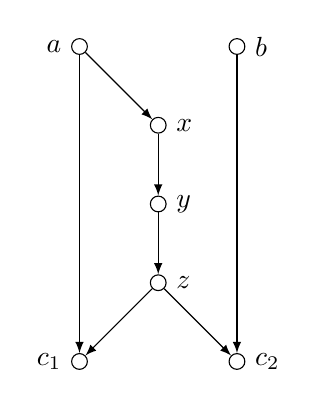
\begin{tikzpicture}
    [
    point/.style={circle,draw,inner sep=0pt,minimum size=2mm}
    ]
    \node (a) at (0,4) [point, label=left:$a$] {};
    \node (x) at (1,3) [point, label=right:$x$] {};
    \node (y) at (1,2) [point, label=right:$y$] {};
    \node (z) at (1,1) [point, label=right:$z$] {};
    \node (c1) at (0,0) [point, label=left:$c_1$] {};
    \node (c2) at (2,0) [point, label=right:$c_2$] {};
    \node (b) at (2,4) [point, label=right:$b$] {};
    \draw [-latex] (a) to (c1);
    \draw [-latex] (a) to (x);
    \draw [-latex] (x) to (y);
    \draw [-latex] (y) to (z);
    \draw [-latex] (z) to (c1);
    \draw [-latex] (z) to (c2);
    \draw [-latex] (b) to (c2);
  \end{tikzpicture}
  \caption{}
  \label{fig:v2_counter_graph}
\end{figure}
\FloatBarrier
Given the above graph, $\ol{ab}$ can be proven like follows:\par
\begin{figure}[!h]
  \centering
  \begin{prooftree*}
    \Hypo{\ol{ax}}
    \Hypo{\ol{yz}}
    \Infer[left label=$xy$]2{\ol{az}}
    \Hypo{\ol{ac_1}}
    \Hypo{\ol{bc_2}}
    \Infer[right label=$zc_1c_2$]3{\ol{ab}}
  \end{prooftree*}
  \caption{}
  \label{fig:v2_counter_proof}
\end{figure}
To show that the graph in Figure~\ref{fig:v2_counter_graph} is not an instance of $V_2$ demands a closer look at the graph.

Assume $V_2(a,b)$.
Since $a$ and $b$ are not connected by an edge, their relation has to be an instance of the inductive step.
Because of the nonemptiness requirement, $\exists c \in N(a):\exists d \in N(c): V_2(d,b)$ from the $V_2$ defintion, either $a$  must have a successor $c$ which again has a successor $d$ such that $V_2(d,b)$ or $b$ must have a successor $c$ which again has a successor $d$ such that $V_2(d,a)$.

The vertices $a$ and $b$ have a total of 3 successors, 2 of which are sinks and therefore unable to satisfy the nonemptiness requirement.
The last successor is the vertex $x$, which only has one successor, vertex $y$.\par
\begin{figure}[!h]
  \centering
  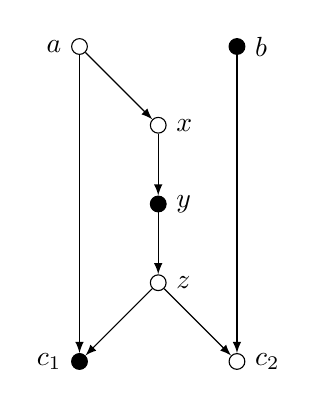
\begin{tikzpicture}
    [
    point/.style={circle,draw,inner sep=0pt,minimum size=2mm},
    one/.style={fill=black}
    ]
    \node (a) at (0,4) [point, label=left:$a$] {};
    \node (x) at (1,3) [point, label=right:$x$] {};
    \node (y) at (1,2) [point,one, label=right:$y$] {};
    \node (z) at (1,1) [point, label=right:$z$] {};
    \node (c1) at (0,0) [point,one, label=left:$c_1$] {};
    \node (c2) at (2,0) [point, label=right:$c_2$] {};
    \node (b) at (2,4) [point,one, label=right:$b$] {};
    \draw [-latex] (a) to (c1);
    \draw [-latex] (a) to (x);
    \draw [-latex] (x) to (y);
    \draw [-latex] (y) to (z);
    \draw [-latex] (z) to (c1);
    \draw [-latex] (z) to (c2);
    \draw [-latex] (b) to (c2);
  \end{tikzpicture}
  \caption{}
  \label{fig:v2_counter_assignment}
\end{figure}
\FloatBarrier
The above solution shows us by soundness of Neg that $\ol{yb}$ is unprovable, and therefore by implication (1) that $y$ and $b$ cannot be $V_2$-related.
Since none of the successors of $a$ and $b$ satisfies the nonemptiness requirement, they also are not $V_2$ related.
We can therefore conclude that $V_2$ does not satisfy implication (2).

Now, in what way can $V_2$ be generalized in order to include the graph in Figure~\ref{fig:v2_counter_graph}?
Looking at the proof in Figure~\ref{fig:proof_v2}, we see that the axiomatic NAND-clause $\ol{ac}$ is a crucial part of the premise, representing the $c \in N(a)$ in the definition of $V_2$.
Observe that a case where $\ol{ac}$ is non-axiomatic would not invalidate this rule application.
In other words, the vertex $c$ from the $V_2$ definition does not necessarily need to be in the neighborhood of $a$, they only need to be in a $V_2$-relation.

Based on this observation, we define the construction $V_3$ which is a generalization of $V_2$.
Like in the definitions of $V_1$ and $V_2$, $a$ and $b$ are vertices from $G$.
\begin{align}
  \textbf{(BC):}&\quad N(a,b) \vee N(b,a) &\Rightarrow V_3(a,b)\label{eq:V2_BC}\\
  \textbf{(IS):}&\quad \exists c \in G:
  \left ( \begin{tabular}{l}
  $\exists d \in N(c) \cup \{ c \} : V_3(d,a) \quad \wedge$\\
  $\exists d \in N(c) \cup \{ c \} : V_3(d,b) \quad \wedge$\\
  $\forall d \in N(c) \cup \{ c \} : V_3(d,a) \vee V_3(d,b) \vee V_3(d,d)$
  \end{tabular} \right )
  &\Rightarrow V_3(a,b)\label{eq:V2_IS}
\end{align}
$V_2$ required $a$ to have an edge to $c$.
We are now treating $c$ just like its successors by requiring it to be in $V_3$-relation to either $a$, $b$ or itself.
Requiring $a$ to be in $V_3$-relation to some vertex in $N(c) \cup \{ c \}$ is now what ensures the inclusion of $a$ in the proof.

Looking back at the graph from Figure~\ref{fig:v2_counter_graph}, we see that vertex $z$ is clearly $V_3$-related to $a$ while its successors, $c_1$ and $c_2$, are $V_3$-related to $a$ and $b$, respectively.
The vertices $a$ and $b$ are thus $V_3$-related.

The proof that $V_3$ satisfies implication (1) is done in much the same way as for $V_2$.
Let $D = N(c) \cup \{ c \}$ and let $D_a$, $D_b$ and $D_d$ denote the same sets as in the $V_2$ proof.
The definition of $V_3$ tells us that both $D_a$ and $D_b$ are now nonempty.
The fact that $D = D_a \cup D_b \cup D_d$ still stands, letting us form the following proof:\par
\begin{figure}[!h]
  \centering
  \begin{prooftree*}
    \Hypo{ \{ \ol{da} \;|\; d \in D_a \} }
    \Hypo{ \{ \ol{db} \;|\; d \in D_b \} }
    \Hypo{ \{ \ol{d} \;|\; d \in D_d \} }
    \Infer[right label=$D$]3{\ol{ab}}
  \end{prooftree*}
  \caption{}
  \label{fig:proof_v3}
\end{figure}
